\section{Model Taxonomy \& Decision Framework}

\begin{frame}{Looking Back: What Have We Built?}
  \begin{center}
    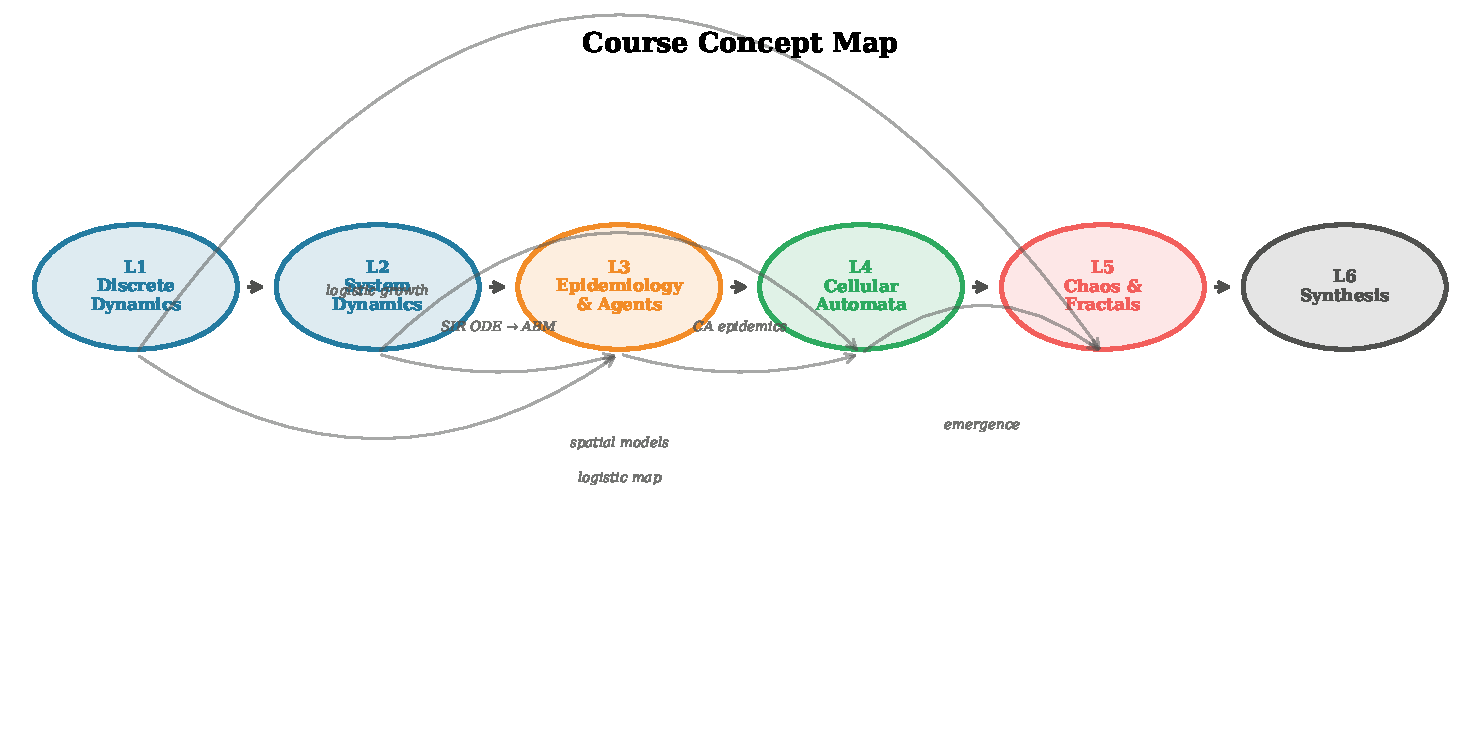
\includegraphics[width=0.85\textwidth]{images/course_map.pdf}
  \end{center}
  \begin{itemize}
    \item Five lessons, each introducing a different \textbf{modelling paradigm}.
    \item Today we step back and ask: \emph{when should I use which approach?}
  \end{itemize}
\end{frame}

\begin{frame}{The Modelling Landscape}
  \begin{center}
    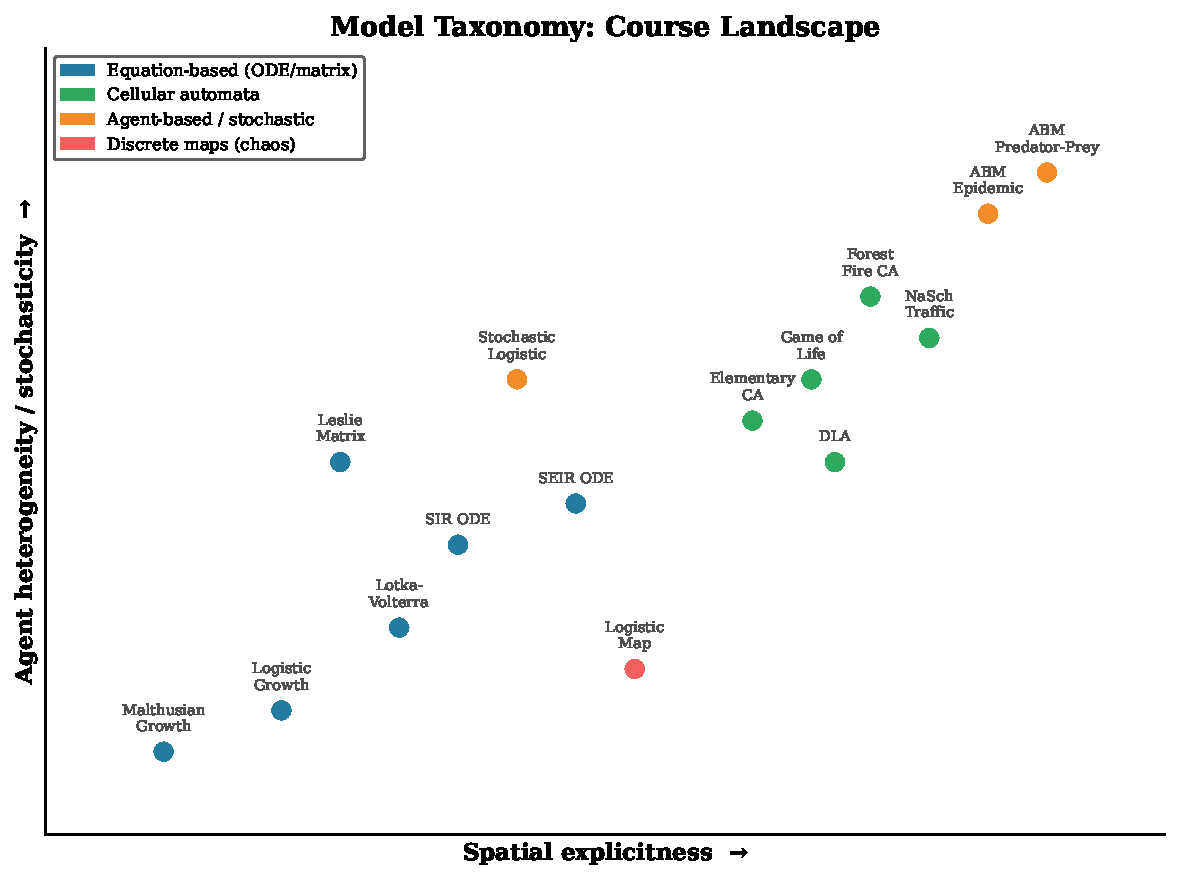
\includegraphics[width=0.78\textwidth]{images/model_taxonomy.pdf}
  \end{center}
  \begin{itemize}
    \item Two key axes: \textbf{spatial explicitness} and \textbf{agent heterogeneity}.
    \item Every model from the course occupies a different region.
  \end{itemize}
\end{frame}

\begin{frame}{Paradigm 1: Equation-Based Models}
  \textbf{What:} Ordinary differential equations (ODEs), difference equations, matrix models.
  \medskip
  \begin{itemize}
    \item Population is described by \textbf{aggregate variables} ($S$, $I$, $R$, $N$).
    \item Individuals are identical and well-mixed.
    \item Time can be continuous (ODE) or discrete (map / matrix).
  \end{itemize}
  \medskip
  \textbf{Course examples:}
  \begin{itemize}
    \item Malthusian \& logistic growth (L1)
    \item Lotka-Volterra predator-prey (L2)
    \item SIR compartmental model (L3)
    \item Leslie matrix (L1)
    \item Logistic map (L5)
  \end{itemize}
\end{frame}

\begin{frame}{Paradigm 2: Cellular Automata}
  \textbf{What:} Grid of cells, each with a discrete state, updated by local rules.
  \medskip
  \begin{itemize}
    \item Space is \textbf{explicit}: a regular lattice.
    \item Time advances in discrete steps.
    \item \textbf{Emergence}: complex global patterns from simple local rules.
    \item No concept of individual ``agents'' --- cells \emph{are} the entities.
  \end{itemize}
  \medskip
  \textbf{Course examples:}
  \begin{itemize}
    \item Conway's Game of Life (L4)
    \item Forest fire model (L4)
    \item Elementary cellular automata (L4)
    \item Nagel-Schreckenberg traffic (project)
  \end{itemize}
\end{frame}

\begin{frame}{Paradigm 3: Agent-Based Models}
  \textbf{What:} Individual agents with their own state, rules, and (often) position.
  \medskip
  \begin{itemize}
    \item Agents can be \textbf{heterogeneous}: different ages, speeds, infection status.
    \item Interactions depend on \textbf{proximity} or \textbf{contact networks}.
    \item Inherently \textbf{stochastic}: randomness in movement, infection, decisions.
    \item Most flexible --- but hardest to analyse mathematically.
  \end{itemize}
  \medskip
  \textbf{Course examples:}
  \begin{itemize}
    \item Agent-based SIR epidemic (L3)
    \item Agent-based predator-prey (L2, project)
    \item Diffusion-limited aggregation (project)
  \end{itemize}
\end{frame}

\begin{frame}{Choosing a Modelling Approach}
  \begin{center}
    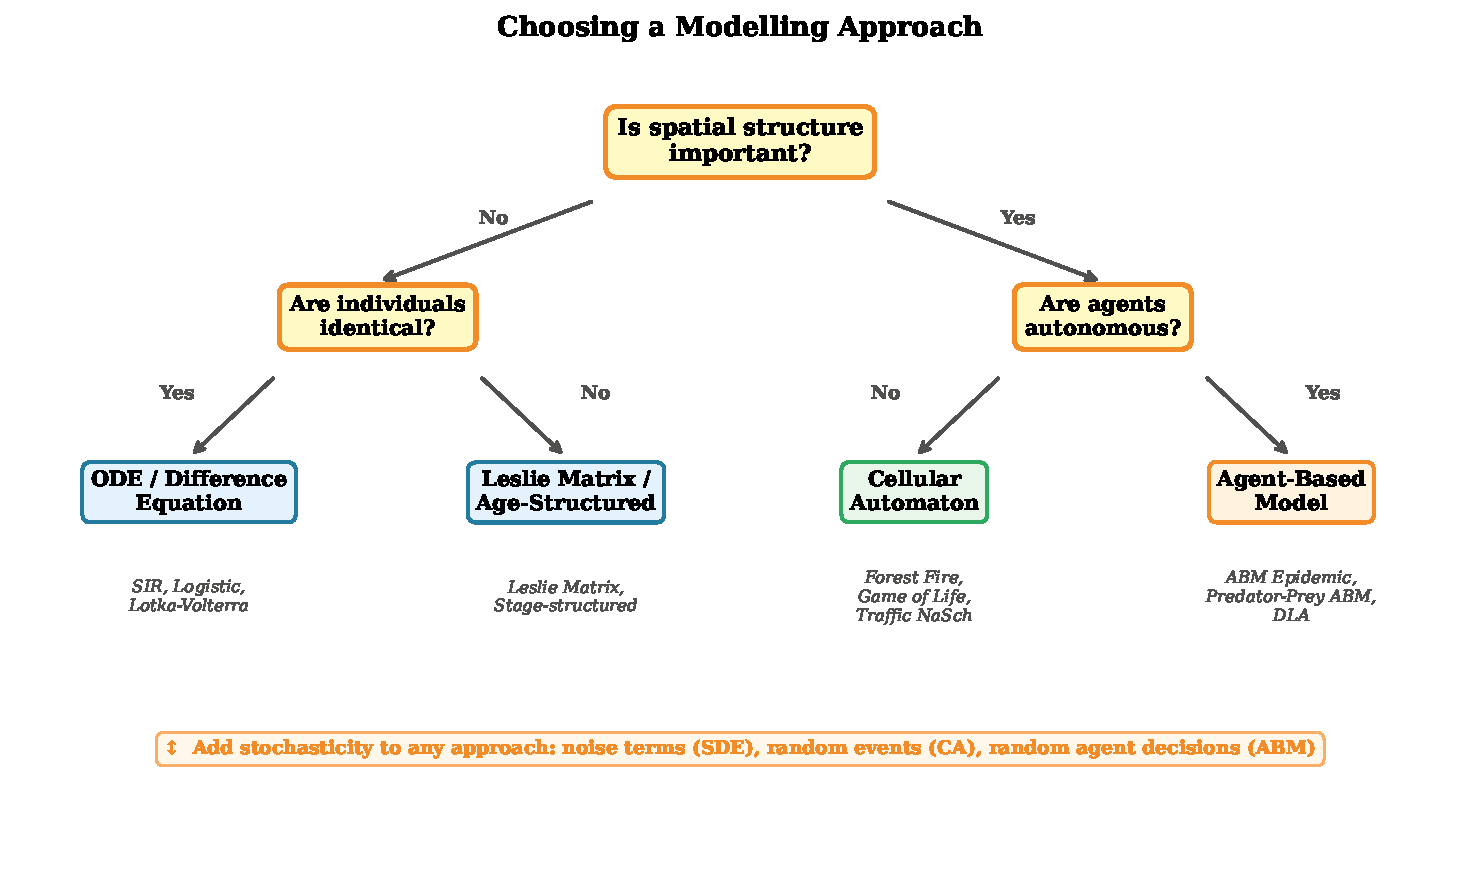
\includegraphics[width=0.82\textwidth]{images/decision_flowchart.pdf}
  \end{center}
\end{frame}

\begin{frame}{Comparing ODE vs ABM: Same System, Different Lens}
  \begin{center}
    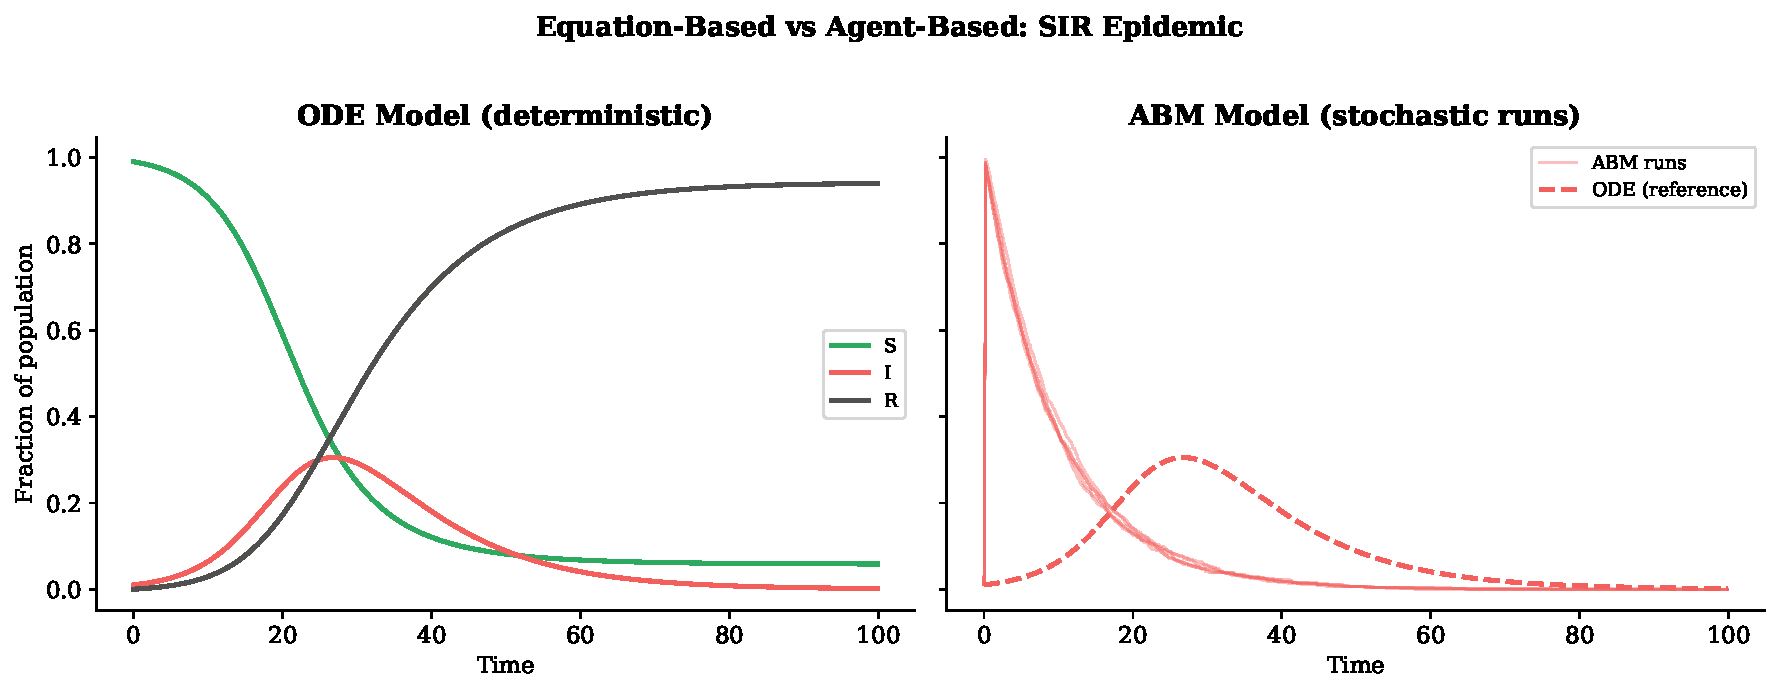
\includegraphics[width=0.95\textwidth]{images/ode_vs_abm_sir.pdf}
  \end{center}
  \begin{itemize}
    \item ODE: smooth, deterministic, fast to compute.
    \item ABM: noisy, captures individual variation, computationally heavier.
    \item \textbf{Key insight}: the ODE is the ``mean-field limit'' of the ABM as $N \to \infty$.
  \end{itemize}
\end{frame}

\begin{frame}{Trade-offs Summary}
  \small
  \begin{center}
  \begin{tabular}{@{}lccc@{}}
    \toprule
    & \textbf{ODE / Matrix} & \textbf{Cellular Automaton} & \textbf{ABM} \\
    \midrule
    Spatial structure   & No  & Grid  & Flexible \\
    Heterogeneity       & No  & Limited  & High \\
    Stochasticity       & Optional (SDE)  & Rule-based  & Inherent \\
    Analytical results  & Often  & Rarely  & Rarely \\
    Computational cost  & Low  & Medium  & High \\
    Interpretability    & High  & Medium  & Lower \\
    \bottomrule
  \end{tabular}
  \end{center}
  \medskip
  \begin{itemize}
    \item There is no single ``best'' approach --- it depends on your \textbf{research question}.
    \item A good strategy: start simple (ODE), add complexity only when needed.
  \end{itemize}
\end{frame}
